\documentclass[12pt]{article}
\usepackage{graphicx}
\usepackage{caption}
\usepackage{subcaption}

\graphicspath{ {fig/} }
\begin{document}
\section{Robot Design}

During the design and assembly stage, two models where proposed. The first prototype used caterpillar wheels, robust body and a sensor on the top with 360$^{\circ}$ of freedom. The second and current model,conversely, is lighter with the sensor suited at the bottom with 180$^{\circ}$ of freedom. It presents the following advantages: 

1) Lightweight. The main robot pieces are the motors, these parts are used as frame to support the body and the NXT control.

2) Compact. The first prototype had a long body because the NXT control was in a horizontal position. This design presented two main problems, difficulties to turn and a considerable error range while rotating. In order to remove these issues the NXT control was placed in vertical position secured by few pieces to the motors.

3) Fast. Taking into account the previous points the robot's movements resulted to be quick and accurate. An improvement was made using a tail to provide more stability and reducing the friction while rotating. 

Images of the final version can be seen in Figure 1.

\begin{figure}[h!]
	\centering
	\begin{subfigure}[b]{0.3\textwidth}
		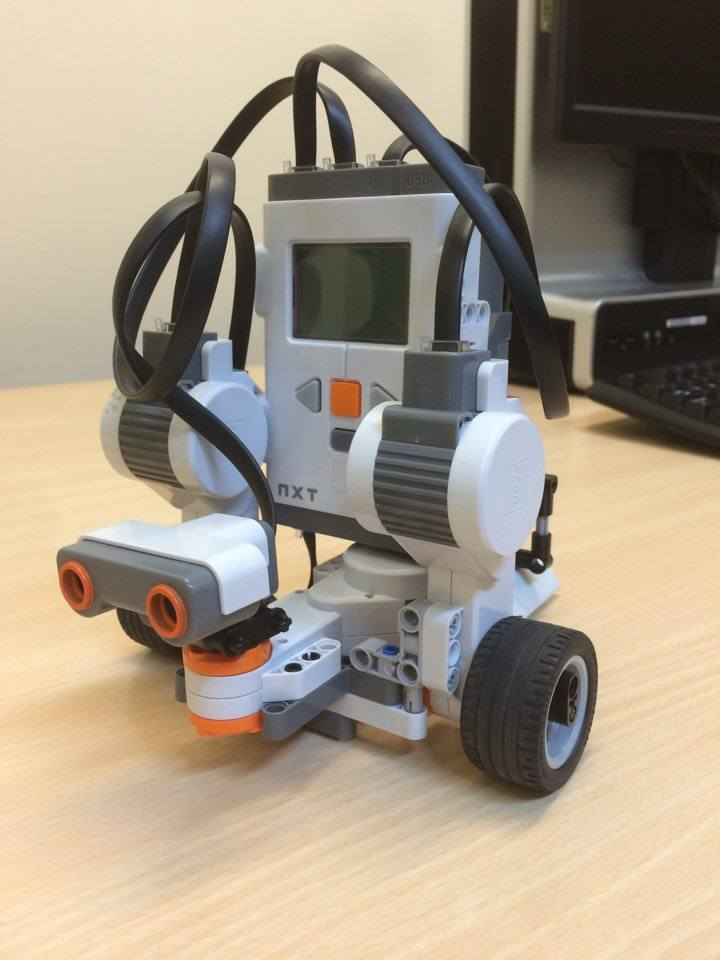
\includegraphics[width=\textwidth]{robot1}
		\caption{Front}
		\label{fig:front}
	\end{subfigure}
	~ %add desired spacing between images, e. g. ~, \quad, \qquad, \hfill etc. 
	%(or a blank line to force the subfigure onto a new line)
	\begin{subfigure}[b]{0.3\textwidth}
		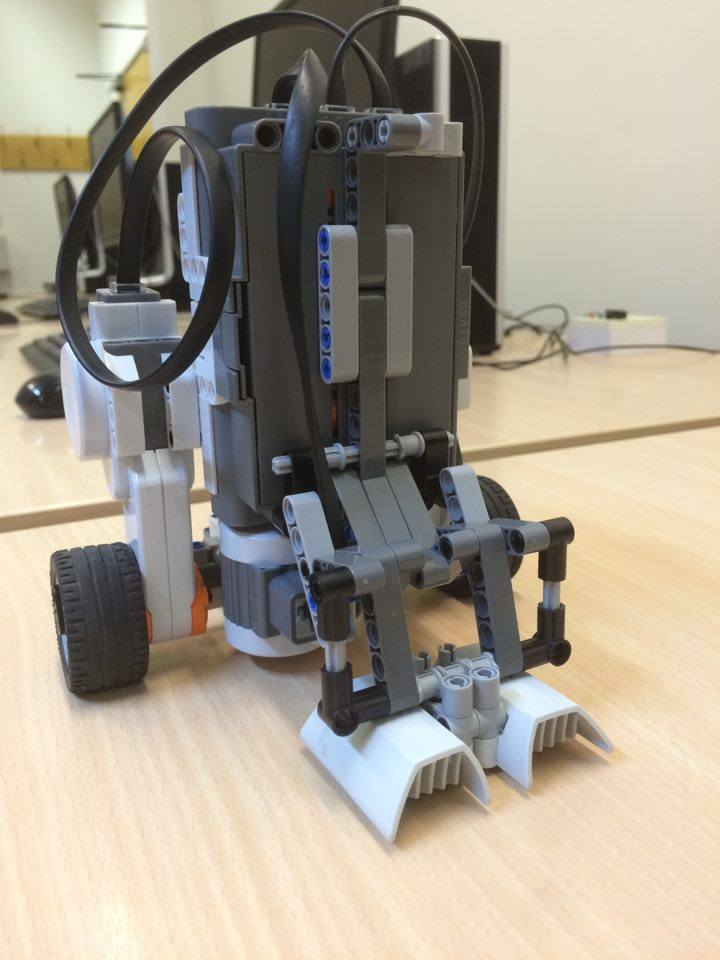
\includegraphics[width=\textwidth]{robot2}
		\caption{Back}
		\label{fig:back}
	\end{subfigure}
	~ 
	\begin{subfigure}[b]{0.3\textwidth}
		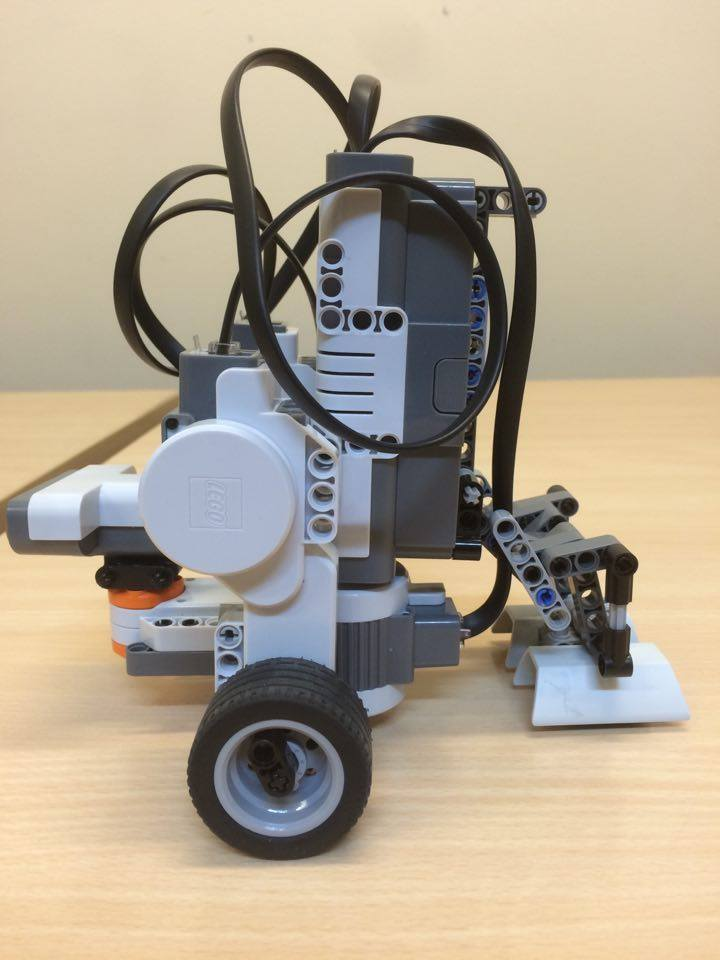
\includegraphics[width=\textwidth]{robot3}
		\caption{Side}
		\label{fig:side}
	\end{subfigure}
	\caption{Robot design views}\label{fig:robot}
\end{figure}

\end{document}